\documentclass[11pt,a4paper]{article}
\usepackage[utf8]{inputenc}
\usepackage{amsmath}
\usepackage{amsfonts}
\usepackage{amssymb}
\usepackage[left=2cm,right=2cm,top=2cm,bottom=2cm]{geometry}


\usepackage{slashed}
\usepackage{hyperref}
\usepackage{graphicx}
\usepackage{caption}
\usepackage{float}
\usepackage{subcaption}

\usepackage{minted}
\usepackage[dvipsnames]{xcolor}


\renewcommand{\theequation}{\arabic{section}.\arabic{equation}}



\usepackage{ifthen}
\usepackage[dvipsnames]{xcolor}
\usepackage{tikz}


%Define color environments:

\newenvironment{DK}[1]{{\color{gray}Commend from D: #1}}

\newenvironment{DKnew}[1]{{\color{blue}NEW from D: #1}}

\newenvironment{DKres}[1]{{\color{BrickRed}RESTRUCTURED from D: #1}}




\newcommand{\dint}{  \displaystyle \int }
%%%%%%%%%%%%%%%%%%%%%%%%%%%%%%%%%%%%%%%%%%
\newcommand{\ie}{{\em i.e.} }
\newcommand{\eg}{{\em e.g.} }
\newcommand{\GeV}{{\rm GeV}}
\newcommand{\TeV}{{\rm TeV}}
\newcommand{\MeV}{{\rm MeV}}
\newcommand{\keV}{{\rm keV}}

\newcommand{\rhs}{RHS }
\newcommand{\lhs}{LHS }


\newcommand{\geff}{ g_{\rm eff} }
\newcommand{\heff}{ h_{\rm eff} }
 
\newcommand{\Ham}{ \mathcal{H} }
 
\newcommand{\thetamax}{ \theta_{\rm max}{} }

 
\newcommand{\thetai}{ \theta_{\rm ini}{} }

\newcommand{\fa}{ f_{\alpha}{} }
 
\newcommand{\ti}{ t_{\rm ini}{} }
 
\newcommand{\Ri}{ R_{\rm ini}{} }


\newcommand{\tosc}{ t_{\rm osc}{} }

\newcommand{\Omegai}{ \Omega_{\rm ini} }
 
\newcommand{\ma}{ m_\alpha{} }

\newcommand{\Lint}{ \mathcal{L}_{\rm int} }


\newcommand{\vev}[1]{\langle #1 \rangle}
\newcommand{\Bvev}[1]{\Bigg\langle #1 \Bigg\rangle}
\newcommand{\bvev}[1]{\Big\langle #1 \Big\rangle}




\newcommand{\lrb}[1]{\left( #1 \right)}
\newcommand{\lrsb}[1]{\left[ #1 \right]}
\newcommand{\lrBigb}[1]{\Big( #1 \Big)}
\newcommand{\lrBigsb}[1]{\Big[ #1 \Big]}
\newcommand{\lrBiggb}[1]{\Bigg( #1 \Bigg)}
\newcommand{\lrBiggsb}[1]{\Bigg[ #1 \Bigg]}

\newcommand{\lrBigcb}[1]{\Big\{ #1 \Big\}}
\newcommand{\lrBiggcb}[1]{\Bigg\{ #1 \Bigg\}}
%%%%%%%%%%%%%%%%%%%%%%%%%%%%%%%%%%%%%%%%%

%%%%%%%%%%%%%%%%%%%%%%%%%%%%%%%%%%%%%%%%%%%%%%%%%%%--Begin_refs--%%%%%%%%%%%%%%%%%%%%%%%%%%%%%%%%%%%%%%%%%%%%%%%%%%%%%%%%%%%%%%%%%%%%%%
\newcounter{NumArgs}

%Define reference to an arbitrary number of equations (\eqs{label_1,label_2....,label_n} will show eqs. ref_1, ref_2, ..., and ref_n)
\newcommand{\eqs}[1]{\setcounter{NumArgs}{0}\foreach\i in{#1}{\stepcounter{NumArgs}}%
\ifthenelse{\equal{\theNumArgs}{1}}{eq.~(\ref{#1})}%
{\ifthenelse{\equal{\theNumArgs}{2}}%
{eqs.~\foreach\i[count=\q]in{#1}{\ifthenelse{\equal{\q}{\theNumArgs}}{and (\ref{\i})}{(\ref{\i})~}}}%
{eqs.~\foreach\i[count=\q]in{#1}{\ifthenelse{\equal{\q}{\theNumArgs}}{and (\ref{\i})}{(\ref{\i}),~}}}}}


%Define reference to an arbitrary number of equations (\Eqs{label_1,label_2....,label_n} will show Eqs. ref_1, ref_2, ..., and ref_n)
\newcommand{\Eqs}[1]{\setcounter{NumArgs}{0}\foreach\i in{#1}{\stepcounter{NumArgs}}%
\ifthenelse{\equal{\theNumArgs}{1}}{Eq.~(\ref{#1})}%
{\ifthenelse{\equal{\theNumArgs}{2}}%
{Eqs.~\foreach\i[count=\q]in{#1}{\ifthenelse{\equal{\q}{\theNumArgs}}{and (\ref{\i})}{(\ref{\i})~}}}%
{Eqs.~\foreach\i[count=\q]in{#1}{\ifthenelse{\equal{\q}{\theNumArgs}}{and (\ref{\i})}{(\ref{\i}),~}}}}}


%Define reference to an arbitrary number of labels (\REF{label_1,label_2....,label_n} will show ref_1, ref_2, ..., and ref_n)
\newcommand{\refs}[1]{\setcounter{NumArgs}{0}\foreach\i in{#1}{\stepcounter{NumArgs}}%
\ifthenelse{\equal{\theNumArgs}{1}}{(\ref{#1})}%
{\ifthenelse{\equal{\theNumArgs}{2}}%
{\foreach\i[count=\q]in{#1}{\ifthenelse{\equal{\q}{\theNumArgs}}{and (\ref{\i})}{(\ref{\i})~}}}%
{\foreach\i[count=\q]in{#1}{\ifthenelse{\equal{\q}{\theNumArgs}}{and (\ref{\i})}{(\ref{\i}),~}}}}}



%Define reference to an arbitrary number of figs (\Figs{label_1,label_2....,label_n} will show ref_1, ref_2, ..., and ref_n)
\newcommand{\Figs}[1]{\setcounter{NumArgs}{0}\foreach\i in{#1}{\stepcounter{NumArgs}}%
\ifthenelse{\equal{\theNumArgs}{1}}{Fig.~(\ref{#1})}%
{\ifthenelse{\equal{\theNumArgs}{2}}%
{Figs.~\foreach\i[count=\q]in{#1}{\ifthenelse{\equal{\q}{\theNumArgs}}{and (\ref{\i})}{(\ref{\i})~}}}%
{Figs.~\foreach\i[count=\q]in{#1}{\ifthenelse{\equal{\q}{\theNumArgs}}{and (\ref{\i})}{(\ref{\i}),~}}}}}




%Define reference to an arbitrary number of "general reference" (\Gen{message}{label_1,label_2....,label_n} will show message.(ref_1), (ref_2), ..., and (ref_n)
\newcommand{\Gen}[2]{\setcounter{NumArgs}{0}\foreach\i in{#2}{\stepcounter{NumArgs}}%
	\ifthenelse{\equal{\theNumArgs}{1}}{#1.~(\ref{#2})}%
	{\ifthenelse{\equal{\theNumArgs}{2}}%
		{#1.~\foreach\i[count=\q]in{#2}{\ifthenelse{\equal{\q}{\theNumArgs}}{and (\ref{\i})}{(\ref{\i})~}}}%
		{#1.~\foreach\i[count=\q]in{#2}{\ifthenelse{\equal{\q}{\theNumArgs}}{and (\ref{\i})}{(\ref{\i}),~}}}}}


%%%%%%%%%%%%%%%%%%%%%%%%%%%%%%%%%%%%%%%%%%%%%%%%%%%--End_refs--%%%%%%%%%%%%%%%%%%%%%%%%%%%%%%%%%%%%%%%%%%%%%%%%%%%%%%%%%%%%%%%%%%%%%%



%%%%%%%-----------------------Rules-----------------------%%%%%%%
% 1. Put any new macros in macros.tex.

% 2. Section should start with:
	%\section{This is a section}\label{sec:Intro}
	%\setcounter{equation}{0}

% 3. labels for Figs should start with fig:, for equations should start with eq:, for sections with sec:, etc.
%%%%%%%--------------------------------------------------%%%%%%%




\author{Karamitros Dimitrios}
\title{{\tt MiMeS}: Misalignment Mechanism Solver}
\begin{document}

\maketitle

\begin{abstract}
	We introduce a \CPP header-only library that solves the Axion equation of motion, \mimes.  
	\mimes makes no assumptions regarding the cosmology and the thermal mass of the axion, which allows the user 
	to consider various cosmological scenarios and axion-like models.
	Moreover, although is written entirely in \CPP, \mimes comes with a convenient \PY interface, which does not require the
	user to write any code in \CPP.
\end{abstract}


\section{Introduction}\label{sec:intro}
\setcounter{equation}{0}

About the axion...

\section{Axion relic abundance}\label{sec:abundance}
\setcounter{equation}{0}
%
Although there are several works in the literature that (such as~\cite{Chang:1998ys}) that can also provide a useful insight on the solution of the axion equation of motion (EOM), it would be useful to derive and define the quantities we need in this section, in order to understand how \mimes works in detail.

\paragraph{The EOM} The axion field is written as 
%
\begin{equation}
	\alpha  \equiv \fa \ \theta,
	\label{eq:fa_def}
\end{equation}
%
with $\fa$ the scale of the axion that determines the the scale at which the PQ symmetry breaks. 

The EOM in terms of $\theta$ is 
%
\begin{equation}
	\lrb{\dfrac{d^2}{d t} + 3 H(t) \ \dfrac{d}{d t} } \theta(t) + m_{\alpha}^2(t) \ \sin \theta(t) = 0 \; ,
	\label{eq:eom}
\end{equation}
%
with $H(t)$ the Hubble parameter (determined by the cosmology), and $m_{\alpha}(t)$  the time (temperature) dependent mass of the axion. 

\paragraph{Initial conditions}
%
\begin{figure}[h!]
	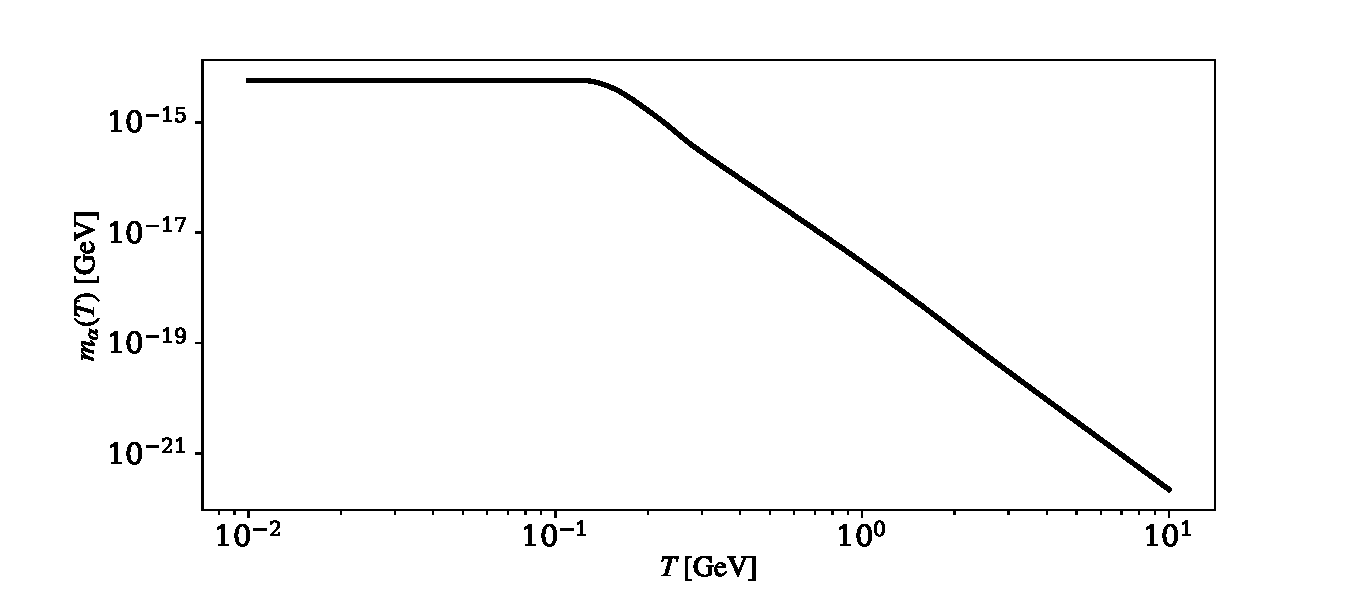
\includegraphics[width=1\textwidth]{figs/axion_mass.pdf}
	\caption{The mass of the axion as a function of the temperature for $\fa=10^{12}~\GeV$, using the data provided in ref.~\cite{Borsanyi:2016ksw}.}
	\label{fig:axion_mass}
\end{figure}
%
Assuming that the PQ symmetry breaks before inflation, the initial conditions (\ie at some $t=0$, after inflation) for the EOM is random. However, we note that $m_{\alpha} \to 0$ (see \Figs{fig:axion_mass}) -- \ie $m_{\alpha} \ll H$ -- at very early times. Therefore, after inflation, the EOM becomes
%
\begin{equation}
	\lrb{\dfrac{d^2}{d t} + 3 H(t) \ \dfrac{d}{d t}  } \theta(t) = 0 \; ,
	\label{eq:massless_eom}
\end{equation}
%
which is solved by $\theta = \thetai + C \dint_{0}^t d t \ \lrb{ \dfrac{R_{0}}{R(t)} }^3$. That is, as the Universe expands, $\theta \approx \thetai$. Since we would like to calculate the relic abundance of axions, we can integrate \eqs{eq:eom} from a time after inflation (call it $t = \ti$) such that $ \dot \theta |_{t=\ti} = 0$ and  $\theta|_{t=\ti} \approx \thetai$.   



\subsection{The WKB approximation}
%
In order to solve analytically \eqs{eq:eom}, we assume $\theta \ll 1$, which results in the linearised EOM
%
\begin{equation}
	\lrb{\dfrac{d^2}{d t} + 3 H(t) \ \dfrac{d}{d t} + m_{\alpha}^2(t) } \theta(t) = 0 \; .
	\label{eq:linear_eom}
\end{equation}

Using a trial solution $\psi = \exp\lrsb{ i \dint d t \ \lrBigb{u(t) +3/2 \ i \ H(t)} }$, and defining $\Omega^2 = m_{\alpha}^2 - \dfrac{9}{4} H^2 -  \dfrac{3}{2} \dot H $ we can transform the \eqs{eq:linear_eom} to 
%
\begin{equation}
	u^2 = \Omega^2 + i \ \dot u \; ,
	\label{eq:eom_of_u}
\end{equation}
%
which has a formal solution $u = \pm \sqrt{\Omega^2 + i \dot u}$. Assuming that $\dot u \ll \Omega^2$ and $\dot \Omega \ll \Omega^2$, we can approximate $u$ as
%
\begin{equation}
	u \approx \pm \Omega + \dfrac{i}{2} \dfrac{d \log \Omega}{d t} \;,
	\label{eq:u_approx}
\end{equation}
%
which results in the general solution of \eqs{eq:linear_eom} 
%
\begin{equation}
	\theta \approx \dfrac{1}{\sqrt{\Omega}} \exp\lrb{-\dfrac{3}{2} \int d t \ H} \lrsb{ A \cos\lrb{ \int d t \ \Omega} +  B \sin\lrb{ \int d t \ \Omega}    } \;. 
	\label{eq:general_solution_eom_approx}
\end{equation}

Applying, then, the initial conditions $ \dot \theta |_{t=\ti} = 0$ and  $\theta|_{t=\ti} \approx \thetai$, we arrive with the solution 
%
\begin{equation}
	\theta(t) \approx \thetai \sqrt{ \dfrac{ \Omegai }{\Omega (t)} } \exp\lrb{-\dfrac{3}{2} \int_{\ti}^t d t^\prime  \ H(t^\prime)} \  \cos\lrb{ \int_{\ti}^t d t^\prime  \ \Omega(t^\prime)}   \;.
	\label{eq:solution_eom_approx} 
\end{equation}


In order to further simplify this approximate result, we note that $\theta$ deviates from $\thetai$ only after the mass becomes comparable to the expansion rate of the Universe, \ie after $m_{\alpha}|_{t = \tosc} = 3 H|_{t = \tosc}$. This observation allows us to use $\ti = \tosc$.  Moreover, at $t> \tosc$, we can approximate $\Omega \approx m_{\alpha}$, as $H^2$ and $\dot H$ become much smaller than $m_\alpha^2$ quickly after $t=\tosc$. Finally, the axion angle takes the form
%
\begin{equation}
	\theta(t) \approx \thetai \lrb{\dfrac{3}{4}}^{1/4} \sqrt{ \dfrac{ \ma|_{t=\tosc} }{\ma  (t)} } \exp\lrb{-\dfrac{3}{2} \int_{\tosc}^t d t^\prime  \ H(t^\prime)} \  \cos\lrb{ \int_{\tosc}^t d t^\prime  \ \ma(t^\prime)}   \;.
	\label{eq:solution_eom_approx_final} 
\end{equation}
%
Notice that we have assumed $\thetai \approx \theta|_{t=\tosc}$ as initial condition, which can impact the accuracy of the WKB approximation, as $\dot \theta|_{t=\tosc} \neq 0$.

\paragraph{Axion energy density}
%
The energy density of the axion is 
%
\begin{eqnarray}
	\rho _\alpha = \dfrac{1}{2} \fa^2 \lrsb{ \dot{\theta}^2 + \ma^2 \theta^2 } \;.
	\label{eq:rho_a_def} 
\end{eqnarray}
%
For the relic abundance of axions, we need to calculate their energy density at very late times. That is, $\dot \ma = 0$, $\ma \gg H$ and $\dot H \ll H^2$. After some algebra, we obtain the approximate form of the energy density (as a function of the scale factor $R$) 
%
\begin{eqnarray}
	\rho _\alpha \approx \dfrac{\ma_{,0} }{2}  \ \fa^2 \ \thetai^2  \ \ma(R_{\rm osc}) \ \lrb{\dfrac{R_{\rm osc}}{R}}^3 \;,
	\label{eq:rho_a0} 
\end{eqnarray}
%
which shows that the energy density of axions at late times scales as the energy density of matter. Thus, today, the energy density of axions can be found by calculating the entropy injection ($\gamma$) between $\tosc$ and today, \ie
%
\begin{equation}
	R^3 \ s = \gamma \ R_{\rm osc}^3 \ s_{\rm osc} \Rightarrow  \lrb{\dfrac{R_{\rm osc}}{R}}^3 = \gamma^{-1} \dfrac{s}{s_{\rm osc}} \;,
\end{equation}
%
which results in the energy density today
\begin{eqnarray}
	\rho _{\alpha,0} = \gamma^{-1}  \dfrac{s_0}{s_{\rm osc}} \  \dfrac{1 }{2}  \ \fa^2 \ \ma_{,0} \ \ma_{,{\rm osc}} \ \thetai^2    \;.
	\label{eq:rho_a_approx} 
\end{eqnarray}
%

\subsection{Adiabatic invariant and the anharmonic factor}\label{sec:an_fac}
%
In oscillatory systems with varying period, the energy is not conserved, and it is usually useful to define an ``adiabatic invariant", which is an approximate constant of motion.

\paragraph{Definition of the adiabatic invariant}
%
Given a system with Hamiltonian $\mathcal{H}(\theta,p;t)$, the equations of motion are 
%
\begin{equation}
	\dot p = - \dfrac{\partial \mathcal{H}}{\partial \theta} \;, \;\; 
	\dot \theta =  \dfrac{\partial \mathcal{H}}{\partial p} \;.
	\label{eq:hamiltonian_eoms}
\end{equation}

Moreover, we note that
%
\begin{equation}
	d \Ham = \dot \theta \ d p - \dot p \ d \theta + \dfrac{\partial \Ham}{\partial t} \ d t \;.  
	\label{eq:total_dH}
\end{equation}


If this system exhibits closed orbits (\eg if it oscillates), we define 
%
\begin{equation}
	J \equiv \oint p \ d \theta \;,
	\label{eq:adiabatic_inv_def}
\end{equation}
%
where the integral is over a closed path (\eg a period, $T$). This quantity is the adiabatic invariant of the system, if the Hamiltonian varies slowly during a cycle. That is,
%
\[
\dfrac{d J}{d t} =  \oint \lrBigb{\dot p \ d \theta + p \ d \dot \theta} = \dint_{t}^{t+T}  \dfrac{\partial \Ham}{\partial t^\prime} \ d t^\prime \approx T \ \dfrac{\partial \Ham(t^{\prime})}{\partial t^{\prime}}\Big|_{t^{\prime}=t} \approx 0 
\;. 
\]
%

It is also noteworthy that this definition can help us identify the time it takes for an orbit to complete, since 
%

\begin{eqnarray}
	&\dfrac{d J}{d t} \approx  T \ \dfrac{\partial \Ham}{\partial t} \Rightarrow \nonumber \\
	&J(t) \approx \Ham(t) \ T + {\rm const.} \Rightarrow \nonumber \\
	&T \approx \dfrac{d J}{d \Ham} \;.  \nonumber 
\end{eqnarray}

\paragraph{Application to the axion}
%
The Hamiltonian that results in the EOM of \eqs{eq:eom} is
%
\begin{equation}
	\Ham = \dfrac{1}{2} \dfrac{p^2}{\fa^2 \ R^3} + V(\theta) \ R^3\;,
	\label{eq:axion_H}
\end{equation}
%
with 
%
\begin{eqnarray}
	& p = \fa^2 \ R^3 \ \dot \theta \\
	\label{eq:momentum}
	& V(\theta) = \ma^2 \fa^2 (1-\cos \theta) \;.
	\label{eq:potential}
\end{eqnarray}

Notice that the Hamiltonian varies slowly if $\dot \ma/\ma \ll \ma$ and $H \ll \ma$, which are the adiabatic conditions.   When these conditions are met, the adiabatic invariant for this system becomes
%
\begin{eqnarray}
	J = & \oint p \ d \theta = \oint \sqrt{ 2\lrb{ \Ham(\theta) - V(\theta) \ R^3} \ \fa^2 R^3 \ }  \ d \theta  =
	\oint \sqrt{ 2\lrb{ \Ham(\thetamax) - V(\theta) \ R^3} \ \fa^2 R^3 \ } d \theta = \nonumber \\ 
	& 2 \int_{- \thetamax} ^{\thetamax}  \sqrt{2}\sqrt{ \lrb{ \Ham(\thetamax) - V(\theta) \ R^3} \ \fa^2 R^3 \ } d \theta =
	\fa 2 \sqrt{2} \int_{- \thetamax} ^{\thetamax}  \sqrt{ V(\theta_{\rm max}) - V(\theta) } R^{3} d \theta = \nonumber \\
	&2\sqrt{2} \ \fa^2 \ \ma \, R^3 \ \dint_{- \thetamax}^{\thetamax} \sqrt{\cos \theta - \cos \thetamax} \ d \theta  
	\;,
	\label{eq:J_axion_derivation}
\end{eqnarray}
%
where we have defined $\thetamax$ the maximum $\theta$ during its oscillation, which corresponds to $p=0$ (by definition). Also, we have used $\Ham(\theta,p) = \Ham(\thetamax,p=0) =  V(\thetamax) \ R^3$ (remember that $\Ham$ is constant during one cycle). Moreover, for the final equality we have used the adiabatic conditions, \ie negligible change of $\ma$ and $R$ during one period.
%

For the sake of consistency with the literature, we define a rescaled adiabatic invariant 
%
\begin{equation}
	I \equiv R^3 \ \ma \ \thetamax^2  \, f(\thetamax)  \;,
	\label{eq:J_axion_def}
\end{equation}
%
where 
\begin{equation}
	f(\thetamax) =\dfrac{ 2 \sqrt{2}}{\pi \thetamax^2 } \dint_{- \thetamax}^{\thetamax} d \theta \sqrt{ \cos \theta - \cos \thetamax } \;,
	\label{eq:anharmonic_f}
\end{equation}
%
is called the anharmonic factor, with $ 0.5 \lesssim f(\thetamax) \leq 1$ (see \Figs{fig:anharmonic_factor}).


\begin{figure}[t]
	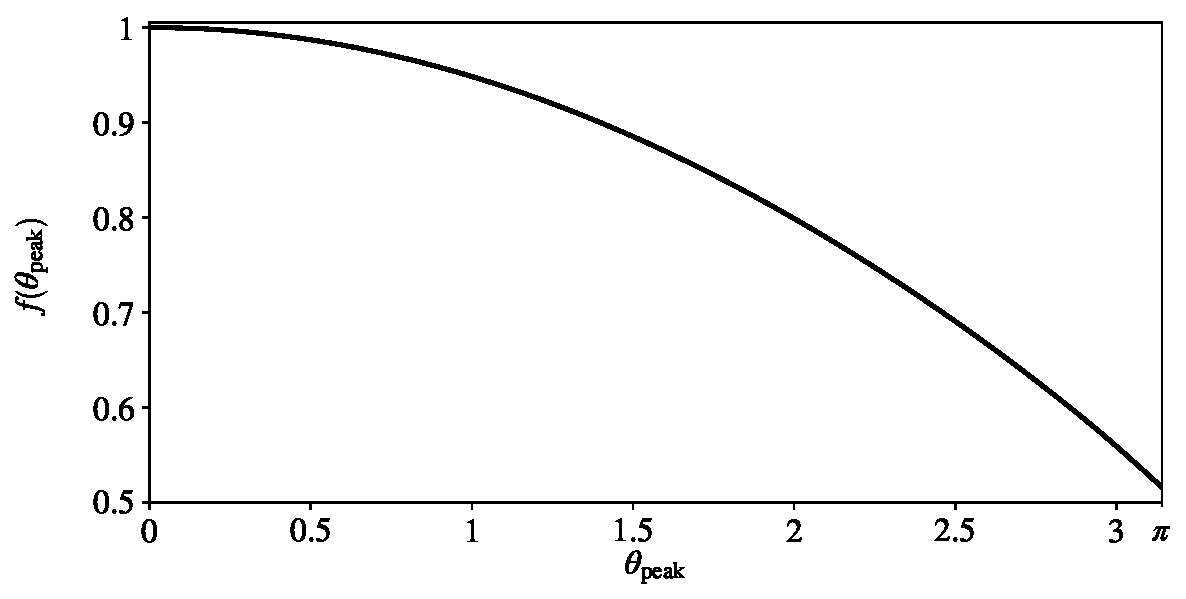
\includegraphics[width=1\textwidth]{figs/anharmonic_factor.pdf}
	\caption{The anharmonic factor for $0 \leq \thetamax < \pi $.}
	\label{fig:anharmonic_factor}
\end{figure}



\paragraph{How to use the adiabatic invariant for numerical calculations}
%
The adiabatic invariant allows us to calculate the maximum value of the angle $\theta$ at late times from its corresponding value at some point after the adiabatic conditions where met. It allows us to calculate the energy density of the axions field taking for $\theta \gtrsim 1$ since we have taken into account the exact potential.


In order to do this, we need to integrate numerically \eqs{eq:eom}, and identify the maxima of $\theta$. Once the adiabatic conditions are fulfilled, we can stop the integration at $\thetamax_{,*}$ (which corresponds to $T_{*}$ and $R_{*}$). Then, the value of the maximum angle today ($\thetamax_{,0} \ll 1$) is related to $\thetamax_{,*}$ via
%
\begin{eqnarray}
	\thetamax_{,0}^2 &=  \lrb{\dfrac{R_*}{R_0}}^3 \ \dfrac{\ma_{,*}}{\ma_{,0}} \ f(\thetamax_{,*}) \ \thetamax_{,*}^2  =
	\gamma^{-1} \ \dfrac{s_0}{s_*} \ \dfrac{\ma_{,*}}{\ma_{,0}} \ f(\thetamax_{,*}) \ \thetamax_{,*}^2 
	\; .
	\label{eq:theta_relation}
\end{eqnarray}
%
Using this, we can determine the energy density of axions today  from \eqs{eq:rho_a_def}. That is,
%
\begin{equation}
	\rho_{\alpha,0} = \gamma^{-1} \ \dfrac{s_0}{s_*} \ \ma_{,0} \ \ma_{,*} \ \dfrac{1}{2} \ \fa^2 \ \thetamax_{,*}^2 \;  \ f(\thetamax_{,*}) \;.
	\label{eq:rho_axion_exact}
\end{equation}
%
Notice that this is similar to the result using the WKB approximation~\ref{eq:rho_a_approx} multiplied by the anharmonic factor, with $\tosc \to t_*$.


\subsection{Notation}\label{sec:beyond_WKB}
%
The WKB approximation is very useful in order to understand the evolution of the axion field. However, it fails to explain how the oscillation begins before $\dot \Omega \ll \Omega^2$ is reached. In this section we will try to understand the evolution of the axion as generally as possible. 


%
The EOM~\ref{eq:eom} depends on time, which is not very useful in cosmology. Therefore, we introduce 
%
\begin{eqnarray}
	u = -\log \dfrac{\Ri}{R} \;,
	\label{eq:natation}
\end{eqnarray}
%
which gives us 
%
\begin{eqnarray}
	&\dfrac{d F}{dt} &=  H  \dfrac{d F}{du} 
	\nonumber \\
	&\dfrac{d^2 F}{dt^2} &= H^2 \ \lrb{ \dfrac{d^2 F}{du^2} + \dfrac{1}{2} \dfrac{d \log H^2}{du}  \dfrac{d F}{du} }\;.
	\label{eq:deriv_u}
\end{eqnarray}

The EOM in terms of $u$, then, becomes
%
\begin{equation}
	\dfrac{d^2  \theta}{du^2} + \lrsb{\dfrac{1}{2} \dfrac{d \log H^2}{du} + 3 } \dfrac{d  \theta}{d u} + \ \lrb{\dfrac{\ma}{H}}^2 \ \sin \theta
	=0 \;.
	\label{eq:eom_u}
\end{equation}

Notice that in a radiation dominated Universe
%
$$
\dfrac{d \log H^2}{du} = -\lrb{ \dfrac{d \log g_*}{d \log T} +4 } \delta_h^{-1}\;,
$$
with  $ \delta_h = 1+ \dfrac{1}{3} \dfrac{d \log h}{d \log T} $.%, such that $\dfrac{d s}{d T} = \delta_h \dfrac{3 \ s}{T}$. 

In general, away from particle annihilations, the expansion rate is dominated by an energy density that scales as $\rho \sim R^{-c}$, \ie $\dfrac{d \log H^2}{du}  = -c$ (for example, for radiation domination $c=4$). 


\paragraph{Behaviour close to the initial condition}
%
Now that we have found the initial conditions, it would be useful to find if $\theta$ tends to increase or decrease once the mass is turned on. For this, we look at time $t = \delta t$, with 
%
\begin{equation*}
	\ddot{\theta} \approx \dfrac{\dot \theta (\delta t)  - \dot \theta (\ti)}{ \delta  t } =  \dfrac{\dot \theta (\delta t)  }{\delta  t } \;.
\end{equation*} 
%
\begin{equation*}
	\dot{\theta} \approx  - \dfrac{\delta t}{1+3 \ H \ \delta t} \  \ma^2  \sin \theta  \approx  - \dfrac{\delta t}{1+3 \ H \ \delta t} \  \ma^2  \sin \thetai\;,
\end{equation*} 
%
which means that $\dot\theta<0$, \ie the angle $\theta$ decreases (if $\thetai>0$) once the mass is activated. Expressing $\dot \theta(\delta t) = \dfrac{\theta - \thetai}{\delta t}$, we can also write
%
\begin{eqnarray}
	\theta & \approx & \thetai -\dfrac{\delta t^2}{1+3 \ H \ \delta t} \  \ma^2  \sin \theta  
	\approx   \thetai - \delta t^2 \ \ma^2 \ \sin \thetai \;, 
	\label{eq:theta_dt}
\end{eqnarray}
%
which indicates that the angle decreases (increases) as the temperature drops if $\thetai>0$ ($\thetai<0$).

Using \eqs{eq:deriv_u}, \eqs{eq:theta_dt} takes the form
%
\begin{eqnarray}
	\theta \approx    \thetai - \delta u^2 \ \lrb{\dfrac{\ma}{H}}_{t=\ti}^2 \ \sin \thetai \;,
	\label{eq:theta_du}
\end{eqnarray}
%
which can be used to estimate the angle at the oscillation temperature
%
\begin{eqnarray}
	\theta_{\rm osc} \approx    \thetai -  \lrb{\dfrac{\ma}{H}}_{t=\ti}^2 \lrsb{ \lrb{\dfrac{h_{\rm osc}}{\gamma_{\rm osc} \ h_{\rm ini}}}^{1/3} \dfrac{T_{\rm osc}}{T_{\rm ini}} -1 } ^{2}   \ \sin \thetai \;,
	\label{eq:theta_osc}
\end{eqnarray}
%
where  $\gamma_{\rm osc}$ the entropy injection between $\Ti$ and $\Tosc$. Notice that in the derivation of \eqs{eq:solution_eom_approx_final} we used $\theta_{\rm osc} = \thetai$ as our first approximation. Thus, \eqs{eq:theta_osc} provides a correction that takes into account the deviation between $\theta_{\rm osc} $ and $ \thetai$, and \eqs{eq:rho_a_approx} becomes (for $\thetai \ll 1$)
%
\begin{eqnarray}
	\rho _{\alpha,0} = \gamma^{-1}  \dfrac{s_0}{s_{\rm osc}} \  \dfrac{1 }{2}  \ \fa^2 \ \ma_{,0} \ \ma_{,{\rm osc}} \ \thetai^2 \lrBiggsb{
		1 -2 \ \lrb{\dfrac{\ma}{H}}_{t=\ti}^2 \  \lrb{\lrb{\dfrac{h_{\rm osc}}{\gamma_{\rm osc} \ h_{\rm ini}}}^{1/3} \dfrac{T_{\rm osc}}{T_{\rm ini}}-1 } ^{2}   }^2    \;,
	\label{eq:rho_a_NLO} 
\end{eqnarray}
%
which implies that the WKB approximation overestimates the energy density of the axion, especially if entropy is being injected close to the oscillation temperature.

\DK{Show examples of relic vs $\thetai$ and relic vs $\thetaosc$ for RD and NSC for bot WKB and numeric. This will help you argue that $\thetaosc$ is needed, \ie \mimes is needed.}


\section{How to start using \mimes}\label{sec:start}
\setcounter{equation}{0}

The library can downloaded from \href{https://github.com/dkaramit/MiMeS}{github.com/dkaramit/MiMeS}. Once download is complete, we can go inside the \mimes directory, and run {\tt bash configure.sh} and  {\tt make}.  The {\tt bash} script {\tt configure.sh}, downloads parts of {\tt NaBBODES} and {\tt SimpleSplines}~\footnote{\href{https://github.com/dkaramit/NaBBODES}{\tt NaBBODES} is header-only library for ODE integration, and \href{https://github.com/dkaramit/SimpleSplines}{\tt SimpleSplines} is header-only library for spline interpolation.}, writes some files, and  makes some directories, needed \mimes. The {\tt makefile} is responsible for compiling some examples and checks, as well as the shared libraries that we need, for the \PY interface.  If everything runs successfully, there should be two new directories {\tt exec} and {\tt lib}. Inside {\tt exec}, there are several executables that we can run, in order to ensure that the code runs (\eg no segmentation fault occurs). For example, {\tt exec/AxionSolve\_check.run}, should print the values of the parameters $\thetai$ and $\fa$, the oscillation temperature and the corresponding value of $\theta$, the evolution of the axion (\eg temperature, $\theta$, $\rho_a$, etc.), and the values of various quantities on the peaks of the oscillation.  In the directory {\tt lib}, there are several shared libraries, that the \PY interface needs.

\paragraph{First steps} There are several examples in \CPP ({\tt Examples/Cpp}) and \PY ({\tt Examples/Python}), as well as \JUPY  notebooks ({Examples/JupyterNotebooks} and {\tt Examples/scan}), that show in detail how \mimes can be used.

\section{Assumptions and user input}\label{sec:assumptions}
\setcounter{equation}{0}

\mimes makes only a few, fairly general, assumptions about the axion. First of all, it is assumed that the axion energy density is always subdominant compared to radiation or any other component of the Universe. Moreover, the initial condition is always taken to be 






\newpage
%%%%%%%%%%%%%%%%%%%%%%%%%%%%%%%
 \bibliography{refs}{}
 \bibliographystyle{JHEP}                        

\end{document}
